% Author: Seongjin Lee 
% Gyeongsang National University, Korea 
% 
% 2021-02-24
%

\documentclass[newPxFont,sthlmFooter,nooffset]{beamer}
\usepackage{kotex}
%\usetheme{sthlm}
\usepackage{../style/beamerthemesthlm}
\hypersetup{pdfauthor={Seongjin Lee (insight@gnu.ac.kr)},
            pdfsubject={Data Structure and Algorithm, Lecture Note},
            pdfkeywords={Data Structure, Algorithm, Lecture, Note},
            pdfmoddate={D: \pdfdate},
            pdfcreator={Seongjin Lee}}

%\setbeamertemplate{footline}[text line]{%
%    \parbox{\linewidth}{\vspace*{-8pt} \insertsectionhead  \hfill\insertshortauthor\hfill\insertpagenumber}}
%\setbeamertemplate{navigation symbols}{}

\usepackage{tkz-graph}

\setbeamertemplate{blocks}[rounded]

\title{Data Structure and Algorithm}
\subtitle{Class 8}
\author[SJL]{Seongjin Lee}
\institute{\href{mailto:insight@gnu.ac.kr}{insight@gnu.ac.kr}\\\url{http://resourceful.github.io}\\Systems Research Lab.\\GNU}
\date{2021-02-24} 

\begin{document}



\frame[plain,t]{\titlepage} 

\frame{\frametitle{Table of contents}\tableofcontents} 


%---------------------------------------------------------
\section{Graph}
\begin{frame}[t]
  \frametitle{First use of Graph}
  \begin{itemize}
  \item Euler used graph to solve the K\"oenigsberg bridge problem in 1736
  \item ``Starting at some land area, is it possible to return to the starting point after walking across each of the bridges exactly once?''
  \end{itemize}
\begin{center}
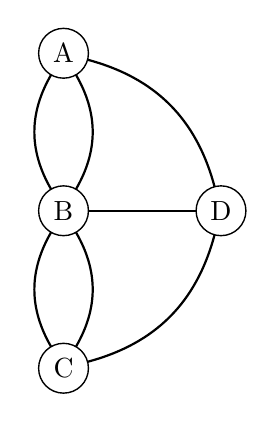
\begin{tikzpicture}
 \SetGraphUnit{2}
 \begin{scope}[rotate=-90]
\Vertex{A}
\EA(A){B}
\EA(B){C}
\NO(B){D}
 \end{scope}
\Edge(B)(D)
\tikzset{EdgeStyle/.append style = {bend left}}
\Edge(A)(B)
\Edge(B)(A)
\Edge(B)(C)
\Edge(C)(B)
\Edge(A)(D)
\Edge(D)(C)
\end{tikzpicture}
\end{center}
\end{frame}


\begin{frame}[t]
  \frametitle{Definitions and Notations}
  \begin{itemize}
  \item \textbf{Notation}: $G=(V,E)$
  \item $V$ is the vertex set. Ex. $V= \{0, 1, 2 ,3\}$
    \begin{itemize}
    \item Vertices are also called nodes and points
    \end{itemize}

  \item $E$ is the edge set. Ex. $E= \{(0,1), (1,3), (2,3), (0, 2)\}$
    \begin{itemize}
    \item Each edge connects two different vertices
    \item Edges are also called arcs and lines
    \end{itemize}

  \end{itemize}


\end{frame}


\begin{frame}[t]
  \frametitle{Directed and Undirected Graphs}
  \begin{itemize}
  \item Directed Edge has an \textit{Orientation} $<u, v>$
    \begin{itemize}
    \item Directed graph (Digraph) = Every Edge has an orientation
    \end{itemize}
  \end{itemize}
  \begin{center}
    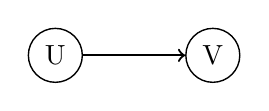
\begin{tikzpicture}
      \GraphInit[vstyle=Normal] 
      \SetGraphUnit{2}
        \Vertex{U}
        \EA(U){V}
      \SetUpEdge[style={->}] 
      \Edge(U)(V)
    \end{tikzpicture}
  \end{center}
  \begin{itemize}
  \item Undirected edge has no \textit{Orientation} $(u, v)$
    \begin{itemize}
    \item Undirected graph = No oriented edge
    \end{itemize}
  \end{itemize}
  \begin{center}
    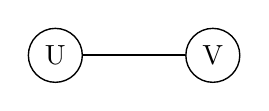
\begin{tikzpicture}
      \GraphInit[vstyle=Normal] 
      \SetGraphUnit{2}
        \Vertex{U}
        \EA(U){V}
      \Edge(U)(V)
    \end{tikzpicture}
  \end{center}
%add sum up -6p KSS-
\begin{itemize}
	\item $(u, v)$ = $(v, u)$ \textbf{but} $<u, v>$ $\ne$ $<v, u>$
\end{itemize}
\end{frame}


\begin{frame}[t]
  \frametitle{Undirected Graph}
  \begin{center}
    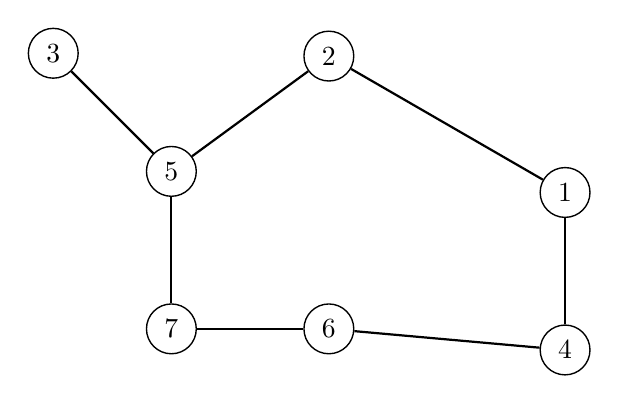
\begin{tikzpicture}
      \GraphInit[vstyle=Normal] 
      \SetGraphUnit{2}
        \Vertices{circle}{1, 2, 6}
        \SO(1){4}
        \WE(6){7}
        \NO(7){5}
      \SetGraphUnit{1.5}
        \NOWE(5){3}
      \Edges(1, 2, 5, 3)
      \Edges(1, 4, 6, 7, 5)
    \end{tikzpicture}\hspace{3em}
    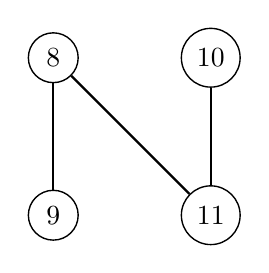
\begin{tikzpicture}
      \GraphInit[vstyle=Normal] 
      \SetGraphUnit{2}
        \Vertex{8}
        \SOEA(8){11}
        \SO(8){9}
        \EA(8){10}
      \Edges(9, 8, 11, 10)
    \end{tikzpicture}
  \end{center}
  \begin{itemize}
  \item $V=\{1, 2, 3, 4, 5, 6, 7, 8, 9, 10, 11\}$
  \item $E=\{(1, 2), (1, 4), (2, 5), (4, 6), (3, 5), (5, 7), (6, 7), (8, 9), (8, 11), (10, 11)\}$
  \end{itemize}
\end{frame}

\begin{frame}[t]
  \frametitle{Directed Graph}
  \begin{center}
    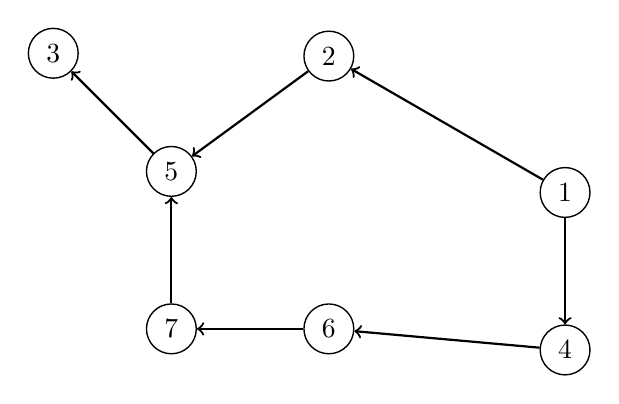
\begin{tikzpicture}
      \GraphInit[vstyle=Normal] 
      \SetGraphUnit{2}
        \Vertices{circle}{1, 2, 6}
        \SO(1){4}
        \WE(6){7}
        \NO(7){5}
      \SetGraphUnit{1.5}
        \NOWE(5){3}
      \SetUpEdge[style={->}]
      \Edges(1, 2, 5, 3)
      \Edges(1, 4, 6, 7, 5)
    \end{tikzpicture}\hspace{3em}
    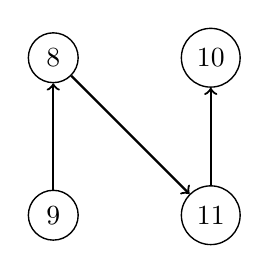
\begin{tikzpicture}
      \GraphInit[vstyle=Normal] 
      \SetGraphUnit{2}
        \Vertex{8}
        \SOEA(8){11}
        \SO(8){9}
        \EA(8){10}
      \SetUpEdge[style={->}]
      \Edges(9, 8, 11, 10)
    \end{tikzpicture}
  \end{center}
  \begin{itemize}
  \item<2-> $V=\{1, 2, 3, 4, 5, 6, 7, 8, 9, 10, 11\}$
  \item<2-> $E=\{<1, 2>, <1, 4>, <2, 5>, <4, 6>, <5, 3>, <6, 7>, <7, 5>, <8, 9>, <8, 11>, <11, 10>\}$
  \end{itemize}
\end{frame}



\begin{frame}[t]
  \frametitle{Applications}
\textbf{Communication Network}
\begin{itemize}
\item Vertex = University
\item Edge = Communication link
\end{itemize}
  \begin{center}
    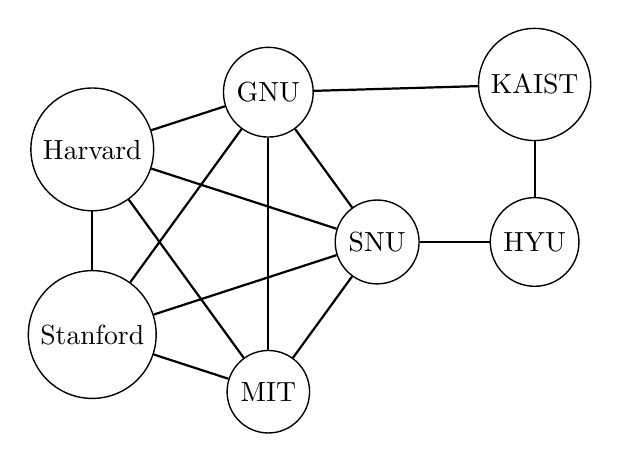
\begin{tikzpicture}
      \GraphInit[vstyle=Normal] 
      \SetGraphUnit{2}
        \Vertices{circle}{SNU, GNU, Harvard, Stanford, MIT}
        \EA(SNU){HYU}
        \NO(HYU){KAIST}
      \SetGraphUnit{1.5}
      \Edges(SNU, GNU, Harvard, Stanford, MIT, SNU)
      \Edges(GNU, Stanford)
      \Edges(Harvard, SNU)
      \Edges(Stanford, SNU)
      \Edges(MIT, GNU)
      \Edges(MIT, Harvard)
      \Edges(SNU, HYU, KAIST, GNU)
    \end{tikzpicture}
  \end{center}
\end{frame}


\begin{frame}[t]
  \frametitle{Applications}
\textbf{Driving Distance/Time Map}
\begin{itemize}
\item Vertex = City
\item Edge Weight = driving distance or time
\end{itemize}
  \begin{center}\vspace{-1em}
    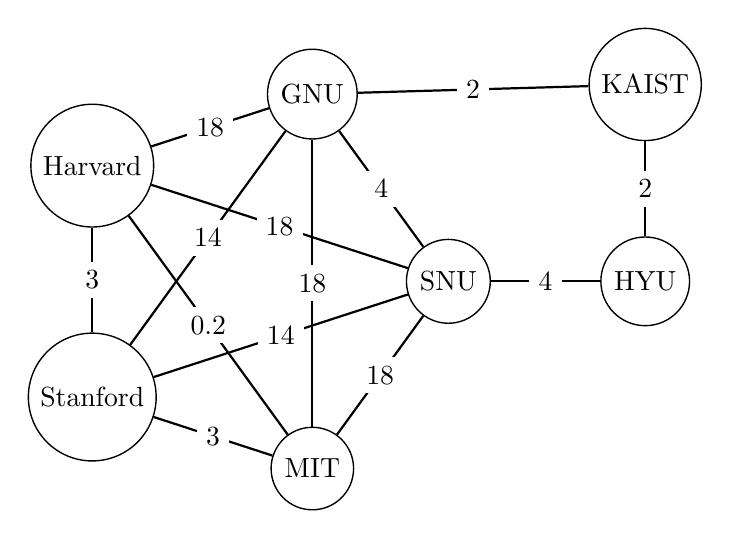
\begin{tikzpicture}
      \GraphInit[vstyle=Normal] 
      \SetGraphUnit{2.5}
        \Vertices{circle}{SNU, GNU, Harvard, Stanford, MIT}
        \EA(SNU){HYU}
        \NO(HYU){KAIST}
      \SetGraphUnit{1.5}
      \Edges[label=4](SNU, GNU)
      \Edges[label=18](GNU, Harvard)
      \Edges[label=3](Harvard, Stanford)
      \Edges[label=3](Stanford, MIT)
      \Edges[label=18](MIT, SNU)
      \Edges[label=14](GNU, Stanford)
      \Edges[label=18](Harvard, SNU)
      \Edges[label=14](Stanford, SNU)
      \Edges[label=18](MIT, GNU)
      \Edges[label=0.2](MIT, Harvard)
      \Edges[label=4](SNU, HYU)
      \Edges[label=2](HYU, KAIST)
      \Edges[label=2](KAIST, GNU)
    \end{tikzpicture}
  \end{center}
\end{frame}


\begin{frame}[t]
  \frametitle{Applications}
Some streets are one way
  \begin{center}
    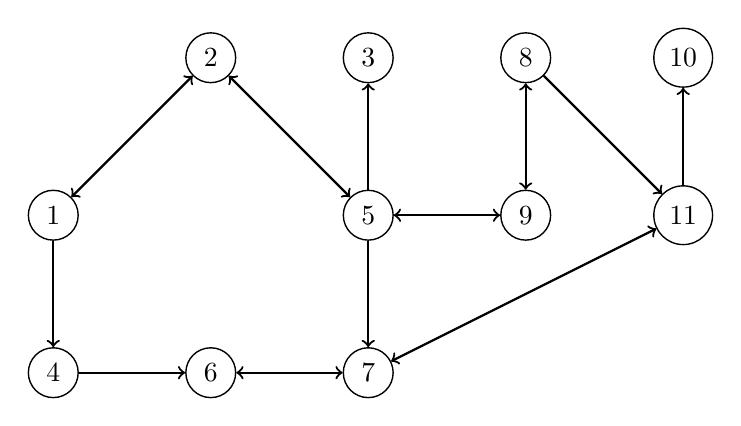
\begin{tikzpicture}
    \GraphInit[vstyle=Normal]\SetGraphUnit{2}
    \Vertex{1}
    \NOEA(1){2}
    \SOEA(2){5}
    \NO(5){3}
    \SO(1){4}
    \EA(4){6}
    \EA(6){7}
    \EA(5){9}
    \NO(9){8}
    \EA(9){11}
    \EA(8){10}
    \Edges[style=<->](1, 2, 5, 9, 8)
    \Edges[style=<->](6, 7, 11)
    \Edges[style=->](1, 4, 6)
    \Edges[style=->](5, 3)
    \Edges[style=->](5, 7)
    \Edges[style=->](8, 11, 10)
    \end{tikzpicture}
  \end{center}

\end{frame}


\begin{frame}[t]
  \frametitle{Complete Undirected Graph}
  \begin{itemize}
  \item A graph that has the maximum number of edges
  \item A graph that has all possible edges
  \end{itemize}

\begin{center}
  \begin{tabular}{c  c  c  c}
    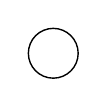
\begin{tikzpicture}
      \GraphInit[vstyle=Normal]\SetGraphUnit{1} \SetVertexNoLabel
      \Vertex{1}
    \end{tikzpicture}
&
  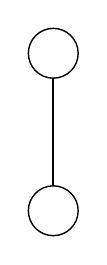
\begin{tikzpicture}
    \GraphInit[vstyle=Normal]\SetGraphUnit{1} \SetVertexNoLabel
    \begin{scope}[rotate=90]
      \Vertices{circle}{1, 2}
    \end{scope}

    \Edges(1,2)
  \end{tikzpicture}
&
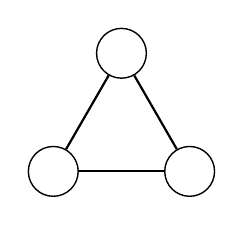
\begin{tikzpicture}
    \GraphInit[vstyle=Normal]\SetGraphUnit{1}
    \SetVertexNoLabel
    \begin{scope}[rotate=90]
      \Vertices{circle}{1, 2, 3}
    \end{scope}

    \Edges(1, 2, 3, 1)
\end{tikzpicture}
&
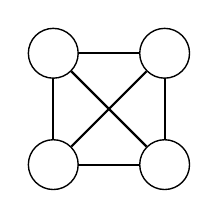
\begin{tikzpicture}
    \GraphInit[vstyle=Normal]\SetGraphUnit{1}
    \SetVertexNoLabel
    \begin{scope}[rotate=45]
      \Vertices{circle}{1, 2, 3, 4}
    \end{scope}

    \Edges(1, 2, 3, 4, 1)
    \Edges(1, 3)
    \Edges(2, 4)
\end{tikzpicture} 
\\
N = 1 & N = 2 & N = 3 & N = 4   
  \end{tabular}
\end{center}
\end{frame}
%add quiz -13p KSS-
\begin{frame}[t]
	\frametitle{Number of Edges in Undirected Graph}
	\begin{itemize}
		\item What is number of edges in this graph ?
	\end{itemize}
\begin{center}
	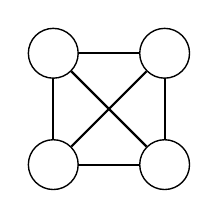
\begin{tikzpicture}
	\GraphInit[vstyle=Normal]\SetGraphUnit{1}
	\SetVertexNoLabel
	\begin{scope}[rotate=45]
	\Vertices{circle}{1, 2, 3, 4}
	\end{scope}
	
	\Edges(1, 2, 3, 4, 1)
	\Edges(1, 3)
	\Edges(2, 4)
	\end{tikzpicture}
	\\
	N = 4 
\end{center}

Number of edges is 6
\end{frame}

\begin{frame}[t]
  \frametitle{Number of Edges in Undirected Graph}
  %typo revised -14p KSS-
  \begin{itemize}
  \item Each edge is of the form $(u, v)$, and $u \neq v$
  \item Number of such pairs in an n vertex graph is $n(n-1)$.
  \item Since edge $(u,v)$ is the same as edge $(v,u)$ the number of edges in a complete undirected graph is $\frac{n(n-1)}{2}$.
  \item Number of edges in an undirected graph is $\leq \frac{n(n-1)}{2}$.
  \end{itemize}
\end{frame}


\begin{frame}[t]
  \frametitle{Number of Edges in Directed Graph}
  \begin{itemize}
  \item Each edge is of the form $<u,v>$, $u \neq v$.
  \item Number of such pairs in an n vertex graph is $n(n-1)$.
  \item Since edge $<u,v>$ is not the same as edge $<v,u>$, the
number of edges in a complete directed graph is $n(n-1)$.
\item Number of edges in a directed graph is $<= n(n-1)$.
  \end{itemize}
\end{frame}


\begin{frame}[t]
  \frametitle{Vertex Degree}
  %typo revised, Degree(5) =3 -> =4 -15p KSS-
  \begin{itemize}
  \item \textbf{Vertex Degree} is the number of edges incident to that vertex
  \item Degree(2) = 2, Degree(5) =4, Degree(3) = 1, 
  \end{itemize}
  \begin{center}
    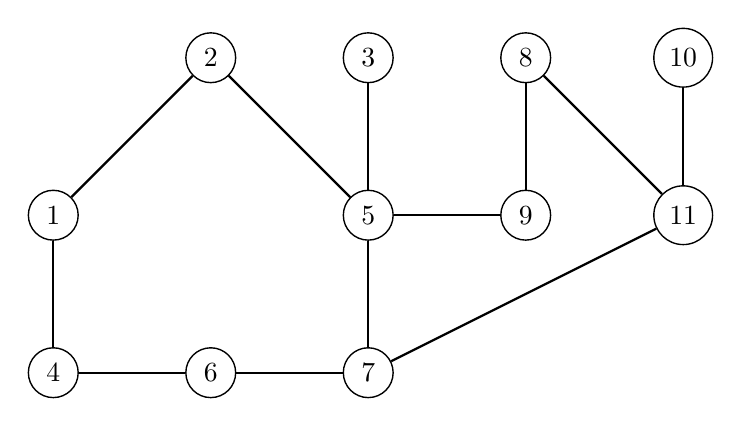
\begin{tikzpicture}
    \GraphInit[vstyle=Normal]\SetGraphUnit{2}
    \Vertex{1}
    \NOEA(1){2}
    \SOEA(2){5}
    \NO(5){3}
    \SO(1){4}
    \EA(4){6}
    \EA(6){7}
    \EA(5){9}
    \NO(9){8}
    \EA(9){11}
    \EA(8){10}
    \Edges(1, 2, 5, 9, 8)
    \Edges(6, 7, 11)
    \Edges(1, 4, 6)
    \Edges(5, 3)
    \Edges(5, 7)
    \Edges(8, 11, 10)
    \end{tikzpicture}
  \end{center}

\end{frame}

\begin{frame}[t]
  \frametitle{Sum of Vertex Degrees}
  \begin{itemize}
  \item \textbf{Sum of Vertex Degrees} is $2\times e$, where $e$ is number of edges
  \end{itemize}
  \begin{center}
    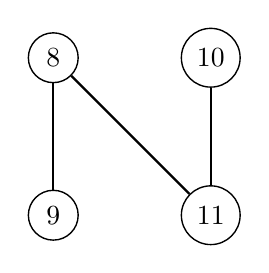
\begin{tikzpicture}
    \GraphInit[vstyle=Normal]\SetGraphUnit{2}
    \Vertex{8}
    \SO(8){9}
    \EA(9){11}
    \EA(8){10}
    \Edges(9, 8, 11, 10)
    \end{tikzpicture}
  \end{center}

\end{frame}


\begin{frame}[t]
  \frametitle{In-Degree of a Vertex}
  \begin{itemize}
  \item In-degree of a vertex is the number of incoming edges
  \item In-degree(2) = 1, in=degree(8) = 0
  \end{itemize}
  \begin{center}
    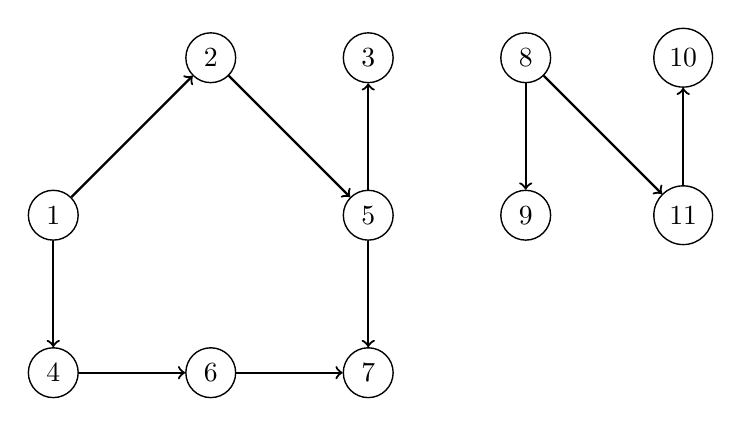
\begin{tikzpicture}
    \GraphInit[vstyle=Normal]\SetGraphUnit{2}
    \Vertex{1}
    \NOEA(1){2}
    \SOEA(2){5}
    \NO(5){3}
    \SO(1){4}
    \EA(4){6}
    \EA(6){7}
    \EA(5){9}
    \NO(9){8}
    \EA(9){11}
    \EA(8){10}
    \Edges[style=->](1, 2, 5, 3)
    \Edges[style=->](5, 7)
    \Edges[style=->](1, 4, 6, 7)
    \Edges[style=->](8, 9)
    \Edges[style=->](8, 11, 10)
    \end{tikzpicture}
  \end{center}

\end{frame}

\begin{frame}[t]
  \frametitle{Out-Degree of a Vertex}
  \begin{itemize}
  \item Out-degree of a vertex is the number of outbound edges
%typo revised -18p KSS-
  \item Out-degree(2) = 1, out-degree(8) = 2
  \end{itemize}
  \begin{center}
    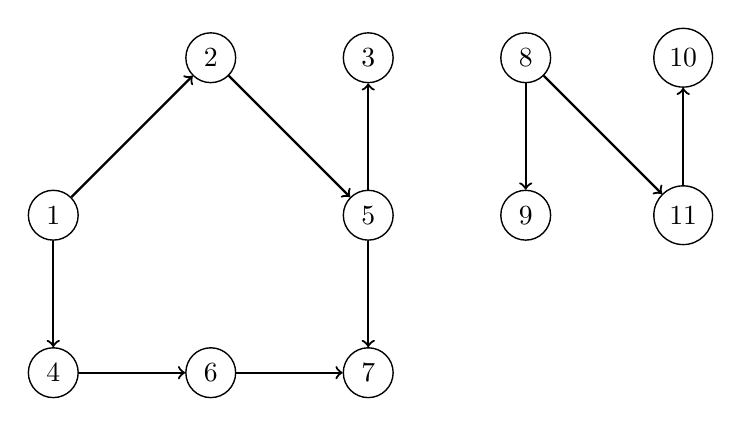
\begin{tikzpicture}
    \GraphInit[vstyle=Normal]\SetGraphUnit{2}
    \Vertex{1}
    \NOEA(1){2}
    \SOEA(2){5}
    \NO(5){3}
    \SO(1){4}
    \EA(4){6}
    \EA(6){7}
    \EA(5){9}
    \NO(9){8}
    \EA(9){11}
    \EA(8){10}
    \Edges[style=->](1, 2, 5, 3)
    \Edges[style=->](5, 7)
    \Edges[style=->](1, 4, 6, 7)
    \Edges[style=->](8, 9)
    \Edges[style=->](8, 11, 10)
    \end{tikzpicture}
  \end{center}

\end{frame}


\begin{frame}[t]
  \frametitle{Sum of In- and Out-Degrees}
  \begin{itemize}
  \item Each edge contributes 1 to the in-degree of some vertex and 1 to the out-degree of some other vertex
  \item Sum of in-degree = sum of out-degree = $e$, where $e$ is the number of edges in the directed graph
  \end{itemize}
\end{frame}


\begin{frame}[t]
  \frametitle{Other Definitions}
  \begin{itemize}
  \item \textbf{Graph}: $G=(V,E)$
  \item  If $G$ is undirected graph and $(u,v)$ is an edge of $G$, then
    \begin{itemize}
    \item $u$ and $v$ are \textbf{adjacent}
    \item $(u,v)$ is \textbf{incident}(부속/교차) on vertices $u$ and $v$
    \end{itemize}

\item If $G$ is directed graph and $<u,v>$ is an edge of $G$, then
  \begin{itemize}
  \item $u$ is \textbf{adjacent} to $v$
  \item $v$ is \textbf{adjacent} from $u$
  \item the edge $<u, v>$ is incident to $u$ and $v$
  \end{itemize}

\item Path from $u$ to $v$
\item \textbf{Simple path} : a path in which all vertices, except
  possibly the first and the last, are distinct (repeats no vertices)
\item \textbf{Cycle} : a simple path in which the first and the last
  vertices are the same
  \end{itemize}
\end{frame}

\section{Graph Representation}
\begin{frame}[t]
  \frametitle{Graph Representation}
  \begin{itemize}
  \item Adjacency Matrix
  \item Adjacency Lists
    \begin{itemize}
    \item Linked Adjacency Lists
    \item Array Adjacency Lists
    \end{itemize}
  \end{itemize}
\end{frame}


\begin{frame}[t]
  \frametitle{Adjacency Matrix}
  \begin{itemize}
  \item $n \times n$ matrix with $0$ and $1$ representing the incidents ,where $n=\#$ of vertices
  \item $A(i, j) = 1$ iff $(i, j)$ is an edge
  \end{itemize}

    \begin{columns}
      \begin{column}{0.4\textwidth}
      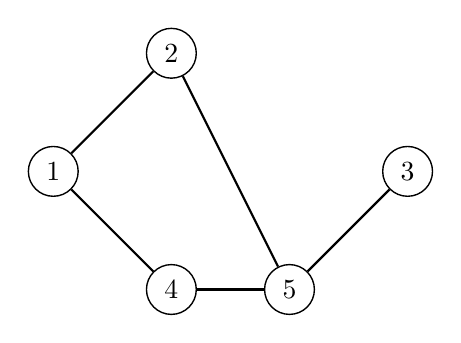
\begin{tikzpicture}
        \GraphInit[vstyle=Normal]
        \SetGraphUnit{1.5}
        \Vertex{1}
        \SOEA(1){4}
        \NOEA(1){2}
        \EA(4){5}
        \NOEA(5){3}
        \Edges(1, 2, 5, 4, 1)
        \Edges(5, 3)
      \end{tikzpicture}
      \end{column}
      \begin{column}{0.4\textwidth}
\begin{tabular}{c | c c c c c }
  ~ & 1 & 2 & 3 & 4 & 5 \\ \hline
  1 & 0 & 1 & 0 & 1 & 0 \\ 
  2 & 1 & 0 & 0 & 0 & 1 \\
  3 & 0 & 0 & 0 & 0 & 1 \\
  4 & 1 & 0 & 0 & 0 & 1 \\
  5 & 0 & 1 & 1 & 1 & 0 
\end{tabular}        
      \end{column}
    \end{columns}
\end{frame}


\begin{frame}[t]
  \frametitle{Properties of Adjacency Matrix}
  \begin{itemize}
  \item Diagonal entries are zero
  \item Adjacency matrix of an undirected graph is symmetric
    \begin{itemize}
    \item $A(i, j) = A(j, i)$ for all $i$ and $j$
    \end{itemize}
  \end{itemize}
    \begin{columns}
      \begin{column}{0.4\textwidth}
      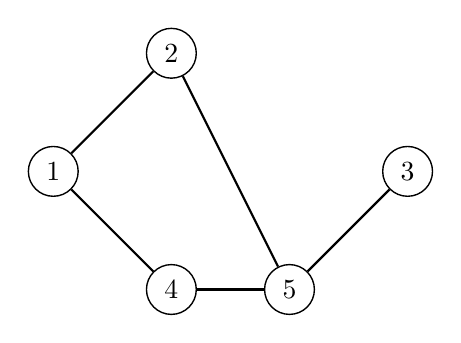
\begin{tikzpicture}
        \GraphInit[vstyle=Normal]
        \SetGraphUnit{1.5}
        \Vertex{1}
        \SOEA(1){4}
        \NOEA(1){2}
        \EA(4){5}
        \NOEA(5){3}
        \Edges(1, 2, 5, 4, 1)
        \Edges(5, 3)
      \end{tikzpicture}
      \end{column}
      \begin{column}{0.4\textwidth}
\begin{tabular}{c | c c c c c }
  ~ & 1 & 2 & 3 & 4 & 5 \\ \hline
  1 & \cellcolor{blue!25}0 & 1 & 0 & 1 & 0 \\ 
  2 & 1 & \cellcolor{blue!25}0 & 0 & 0 & 1 \\
  3 & 0 & 0 & \cellcolor{blue!25}0 & 0 & 1 \\
  4 & 1 & 0 & 0 & \cellcolor{blue!25}0 & 1 \\
  5 & 0 & 1 & 1 & 1 & \cellcolor{blue!25}0 
\end{tabular}        
      \end{column}
    \end{columns}
\end{frame}


\begin{frame}[t]
  \frametitle{Adjacency Matrix for Directed Graph}
  \begin{itemize}
  \item Diagonal entries are zero
  \item Adjacency matrix of a directed graph need not be symmetric
  \end{itemize}
    \begin{columns}
      \begin{column}{0.4\textwidth}
      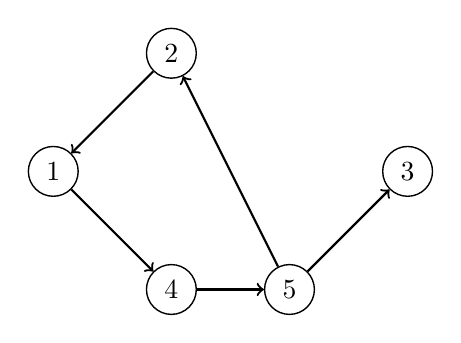
\begin{tikzpicture}
        \GraphInit[vstyle=Normal]
        \SetGraphUnit{1.5}
        \Vertex{1}
        \SOEA(1){4}
        \NOEA(1){2}
        \EA(4){5}
        \NOEA(5){3}
        \Edges[style=->](2, 1, 4, 5, 2)
        \Edges[style=->](5, 3)
      \end{tikzpicture}
      \end{column}
      \begin{column}{0.4\textwidth}
\begin{tabular}{c | c c c c c }
  ~ & 1 & 2 & 3 & 4 & 5 \\ \hline
  1 & \cellcolor{blue!25}0 & 0 & 0 & 1 & 0 \\ 
  2 & 1 & \cellcolor{blue!25}0 & 0 & 0 & 0 \\
  3 & 0 & 0 & \cellcolor{blue!25}0 & 0 & 0 \\
  4 & 0 & 0 & 0 & \cellcolor{blue!25}0 & 1 \\
  5 & 0 & 1 & 1 & 0 & \cellcolor{blue!25}0 
\end{tabular}        
      \end{column}
    \end{columns}
\end{frame}


\begin{frame}[t]
  \frametitle{Properties of Adjacency Matrix}
  \begin{itemize}
  \item $n^2$ bits of space is required
  \item For an undirected graph, may store only lower or upper triangle (exclude the diagonal)
    \begin{itemize}
    \item $\frac{n(n-1)}{2}~bits$
    \end{itemize}
  \item $O(n)$ time to find vertex degree and/or vertices adjacent to a give vertex
  \end{itemize}
\end{frame}


\begin{frame}[t]
  \frametitle{Adjacency Lists}
  \begin{itemize}
  \item Adjacency list for vertex $i$ is a linear list of vertices adjacent from vertex $i$.
  \item An array of $n$ adjacency lists.
  \end{itemize}

    \begin{columns}
      \begin{column}{0.4\textwidth}
      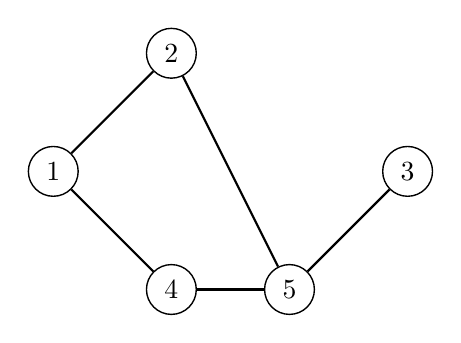
\begin{tikzpicture}
        \GraphInit[vstyle=Normal]
        \SetGraphUnit{1.5}
        \Vertex{1}
        \SOEA(1){4}
        \NOEA(1){2}
        \EA(4){5}
        \NOEA(5){3}
        \Edges(2, 1, 4, 5, 2)
        \Edges(5, 3)
      \end{tikzpicture}
      \end{column}
      \begin{column}{0.4\textwidth}
AdjList[1] = (2, 4) \\
AdjList[2] = (1, 5) \\
AdjList[3] = (5) \\
AdjList[4] = (5, 1) \\
AdjList[5] = (2, 4, 3) \\
      \end{column}
    \end{columns}
\end{frame}


\begin{frame}[t]
  \frametitle{Linked Adjacency Lists}
  \begin{itemize}
  \item Each adjacency list is a chain
    \begin{itemize}
    \item Array length = \texttt{n}
    \item $\#$ of chain nodes = $2e$ (undirected graph)
    \item $\#$ of chain nodes = $e$ (directed graph)
    \end{itemize}
  \end{itemize}
    \begin{columns}
      \begin{column}{0.3\textwidth}
      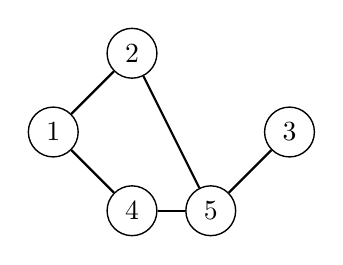
\begin{tikzpicture}
        \GraphInit[vstyle=Normal]
        \SetGraphUnit{1}
        \Vertex{1}
        \SOEA(1){4}
        \NOEA(1){2}
        \EA(4){5}
        \NOEA(5){3}
        \Edges(2, 1, 4, 5, 2)
        \Edges(5, 3)
      \end{tikzpicture}
      \end{column}
      \begin{column}{0.6\textwidth}
      \begin{tikzpicture}
\foreach \index/\list in {1/{2, 4, null}, 2/{1, 5, null}, 3/{5,null}, 4/{5, 1, null}, 5/{2, 4, 3, null}} {
   \node[array element] (aux) at (0,-\index) {\index};
   \LinkedList{\list}
}
      \end{tikzpicture}
      \end{column}
    \end{columns}

\end{frame}


\begin{frame}[t]
  \frametitle{Linked Adjacency Lists}
  \begin{itemize}
  \item Each adjacency list is an array list
    \begin{itemize}
    \item Array length = \texttt{n}
    \item $\#$ of chain nodes = $2e$ (undirected graph)
    \item $\#$ of chain nodes = $e$ (directed graph)
    \end{itemize}
  \end{itemize}
    \begin{columns}
      \begin{column}{0.3\textwidth}
      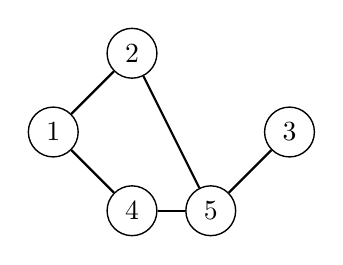
\begin{tikzpicture}
        \GraphInit[vstyle=Normal]
        \SetGraphUnit{1}
        \Vertex{1}
        \SOEA(1){4}
        \NOEA(1){2}
        \EA(4){5}
        \NOEA(5){3}
        \Edges(2, 1, 4, 5, 2)
        \Edges(5, 3)
      \end{tikzpicture}
      \end{column}
      \begin{column}{0.6\textwidth}
      \begin{tikzpicture}
\foreach \index/\list in {1/{2, 4}, 2/{1, 5}, 3/{5}, 4/{5, 1}, 5/{2, 4, 3}} {
   \node[array element] (aux) at (0,-\index) {\index};
   \LinkedListArray{\list}
}
      \end{tikzpicture}
      \end{column}
    \end{columns}

\end{frame}


\begin{frame}[t]
  \frametitle{Weighted Graphs}
  \begin{itemize}
  \item Cost Adjacency Matrix
    \begin{itemize}
    \item $C(i, j) =$ cost of edge $(i, j)$
    \end{itemize}
  \item Each list element of adjacency lists is a pair \texttt{(Adjacent vertex, Edge weight)}
  \end{itemize}
\end{frame}



\end{document}